% =====================================================================
%  Chapter 3 --- Data Understanding (staging-layer only, EDA-enriched)
% =====================================================================
\chapter{Data Understanding through Staging-Layer Profiling}
\label{chap:data}

\section{Introduction}
The previous chapter has defined the architectural target and the technology stack of the platform. The present chapter executes the second phase of the CRISP-DM methodology --- the \emph{data understanding} --- on the analytical PostgreSQL database loaded from the MySQL dumps of \hostorg{}. The scope of this chapter is voluntarily restricted to the \texttt{staging} schema, that is, to the tables produced one-to-one by the MySQL-to-PostgreSQL conversion bridge and \emph{before} any modelling-oriented restructuring. The dimensional warehouse and the analytical marts that consume \texttt{staging} are deliberately deferred to Chapter~\ref{chap:prep}: they are output artefacts of the data preparation phase and not input artefacts of the data understanding phase.

The chapter (i)~describes the three operational MySQL databases that supply the project, (ii)~formalizes the dump-based extraction protocol, (iii)~documents the schema of the resulting staging layer, (iv)~audits the quality of the staging tables with explicit SQL queries, (v)~conducts a complete exploratory data analysis (EDA) on the principal indicators of \texttt{staging.path}, \texttt{staging.rep\_overspeed} and \texttt{staging.notification}, (vi)~profiles the high-frequency telemetry archive \texttt{staging.archive} (about 54.7~million sensor pings, 17~GB on disk) which carries the raw signals reused by the feature-engineering and modelling phases of Chapters~\ref{chap:prep} and~\ref{chap:model}, and (vii)~answers the four analytical questions on which the rest of the report relies: data quality and integrity, stability of the temporal patterns, distribution of the duration target and class imbalance of the status flags. Every figure of this chapter has been generated by the Jupyter notebook \texttt{notebooks/01\_data\_understanding/03\_eda\_chapter3.ipynb} (live MCP queries on PostgreSQL) and rendered by the Python script \texttt{scripts/python/figures/fig\_eda\_chapter3.py} (offline-capable replay). Both scripts query exclusively the \texttt{staging} schema.

\section{Source databases of \hostorg}

\subsection{Three operational MySQL databases}
As described in Chapter~\ref{chap:context}, the operational ecosystem of \hostorg{} relies on three MySQL databases that fulfil complementary roles. The first one --- denoted \emph{raw telemetry} --- collects the binary frames pushed by the GPS/IoT devices through SIM-card connectivity and persists them as \emph{hexadecimal} payloads. The second one --- denoted \emph{decoded archive} --- hosts the readable representation of the telemetry produced by an internal decoding toolchain; its tables follow the naming convention \texttt{arch\_xxxxx} and retain approximately the most recent six months of data. The third one --- denoted \emph{master data} --- carries the customers, drivers, vehicles, contracts and per-tenant configuration; its tables follow the convention \texttt{user\_xxxxx}, with one logical subgroup per tenant.

The present project consumes the second and third databases, namely the decoded \texttt{arch\_xxxxx} archive and the \texttt{user\_xxxxx} master data. The first database --- the raw hexadecimal stream --- is documented for completeness but is not exploited directly: its content has already been transformed by the internal decoding scripts of \hostorg{} before it enters the archive.

\subsection{Tables of interest}
Within the two consumed databases, five families of tables have been retained for the analytical scope of the project: the trip-related family in the archive (\texttt{path}, \texttt{rep\_overspeed}, \texttt{stop}); the alert family (\texttt{notification}); the daily-aggregate family (\texttt{rep\_activity\_daily}); the high-resolution telemetry family in the archive (\texttt{archive}, with about 54.7~million rows over the available history); and the master-data family in the user database (\texttt{vehicule}, \texttt{driver}, \texttt{maintenance}, \texttt{document}, fueling tables). After conversion, these tables populate the \texttt{staging} schema of the analytical PostgreSQL with a faithful one-to-one correspondence: a row in \texttt{arch\_xxxxx.path} becomes a row in \texttt{staging.path}, with the same columns, the same primary key and the same business semantics.

\section{Acquisition strategy}

\subsection{Dump-based extraction from MySQL}
Because the operational databases run on MySQL and are not directly reachable from the analytical environment, the data is acquired through a dump-based protocol. The engineering team of \hostorg{} produces \texttt{.sql} dump files of the relevant slices of the \texttt{arch\_xxxxx} archive and of the \texttt{user\_xxxxx} master data, which are then transferred to the analytical environment. The dumps are converted to a PostgreSQL-compatible representation by the conversion bridge documented in Chapter~\ref{chap:prep}, and finally loaded into the \texttt{staging} schema. This extraction protocol guarantees that the operational MySQL workload is not perturbed by the analytical activity: the load on the production system is bounded to the duration of the dump itself, which is scheduled outside customer-facing peak hours.

\subsection{Connection to the analytical PostgreSQL}
Once the converted dump has been loaded, all subsequent profiling and exploration is performed directly on the \texttt{staging} schema of the analytical PostgreSQL. The connection from a developer notebook to the database follows the standard Python toolchain (\texttt{psycopg2} or SQLAlchemy), through an SSH tunnel terminating on \texttt{localhost:5432} of the Azure VM. Listing~\ref{lst:psycopg-connect} shows the canonical connection snippet.

\begin{lstlisting}[style=python,caption={Read-only connection from Python to the analytical PostgreSQL.},label={lst:psycopg-connect}]
import os
from sqlalchemy import create_engine

PG_DSN = (
    f"postgresql+psycopg2://{os.environ['PG_USER']}:{os.environ['PG_PWD']}"
    f"@{os.environ['PG_HOST']}:{os.environ['PG_PORT']}/{os.environ['PG_DB']}"
)
engine = create_engine(PG_DSN, pool_pre_ping=True, future=True)
\end{lstlisting}

\subsection{MCP-driven exploration}
During the data understanding phase, the Model Context Protocol (MCP) PostgreSQL server has been used as a programmable interface for ad-hoc exploration. Each exploratory question (row counts, null rates, distinct values, distributions) is expressed as an SQL query over the \texttt{staging} schema and submitted to the MCP server, which returns a structured result that is post-processed in the notebooks. This setup substantially accelerates the iteration cycle and standardizes the queries between the two members of the binomial. When the MCP server is unavailable, the same SQL is replayed manually through the Python script \texttt{scripts/python/figures/fig\_eda\_chapter3.py}, whose offline mode embeds a frozen snapshot of every numerical value cited in this chapter.

\section{Schema analysis of the staging layer}

\subsection{Schema inspection queries}
The schema of the \texttt{staging} layer is inspected through the standard catalogue queries on \texttt{information\_schema}. Listing~\ref{lst:schema-columns} shows the canonical query, retrieving for every column its type, its nullability, its default and its ordinal position.

\begin{lstlisting}[style=sql,caption={Schema inspection query against \texttt{information\_schema}, restricted to the \texttt{staging} schema.},label={lst:schema-columns}]
SELECT
    table_name, column_name,
    data_type, is_nullable, column_default, ordinal_position
FROM information_schema.columns
WHERE table_schema = 'staging'
ORDER BY table_name, ordinal_position;
\end{lstlisting}

\subsection{Volumetric profile of the staging tables}
Table~\ref{tab:volumetry} shows the row counts of the principal staging tables, measured by the EDA notebook on the live PostgreSQL database. The figures confirm that the conversion bridge has preserved the original volumetry: the high-frequency telemetry archive \texttt{staging.archive} dominates with about 54.72~million sensor pings (occupying $\sim$17~GB on disk, including indexes), \texttt{staging.path} (the trip table) carries about 7.48~million rows, \texttt{staging.stop} about 12.13~million rows, \texttt{staging.rep\_overspeed} about 1.05~million rows, \texttt{staging.notification} about 0.66~million rows, and \texttt{staging.rep\_activity\_daily} about 63{,}000 rows. The master-data tables (\texttt{vehicule}, \texttt{driver}, \texttt{assignment}) are several orders of magnitude smaller, as expected.

\begin{table}[h]
\centering
\caption{Row counts on the principal staging tables (snapshot 2026-05-06).}
\label{tab:volumetry}
\begin{tabular}{|l|r|r|}
\hline
\textbf{Staging table} & \textbf{Rows} & \textbf{Total size} \\
\hline
\texttt{staging.archive}              & 54{,}720{,}000 & $\sim$17~GB \\
\texttt{staging.stop}                 & 12{,}133{,}639 & --- \\
\texttt{staging.path}                 &  7{,}482{,}166 & --- \\
\texttt{staging.rep\_overspeed}       &  1{,}048{,}936 & --- \\
\texttt{staging.notification}         &    659{,}968 & --- \\
\texttt{staging.rep\_activity\_daily} &     63{,}471 & --- \\
\texttt{staging.driver}               &     \emph{$\sim$thousands} & --- \\
\texttt{staging.vehicule}             &     638 & --- \\
\hline
\end{tabular}
\end{table}

\subsection{Schema map}
The full logical schema of the staging tables is reproduced in Figure~\ref{fig:schema-map}. The map highlights the foreign-key relationships between the trip-related tables of the archive (\texttt{path}, \texttt{stop}, \texttt{rep\_overspeed}), the master-data tables imported from the \texttt{user\_xxxxx} database (\texttt{vehicule}, \texttt{driver}, \texttt{assignment}) and the alert table (\texttt{notification}).

\begin{figure}[h]
\centering
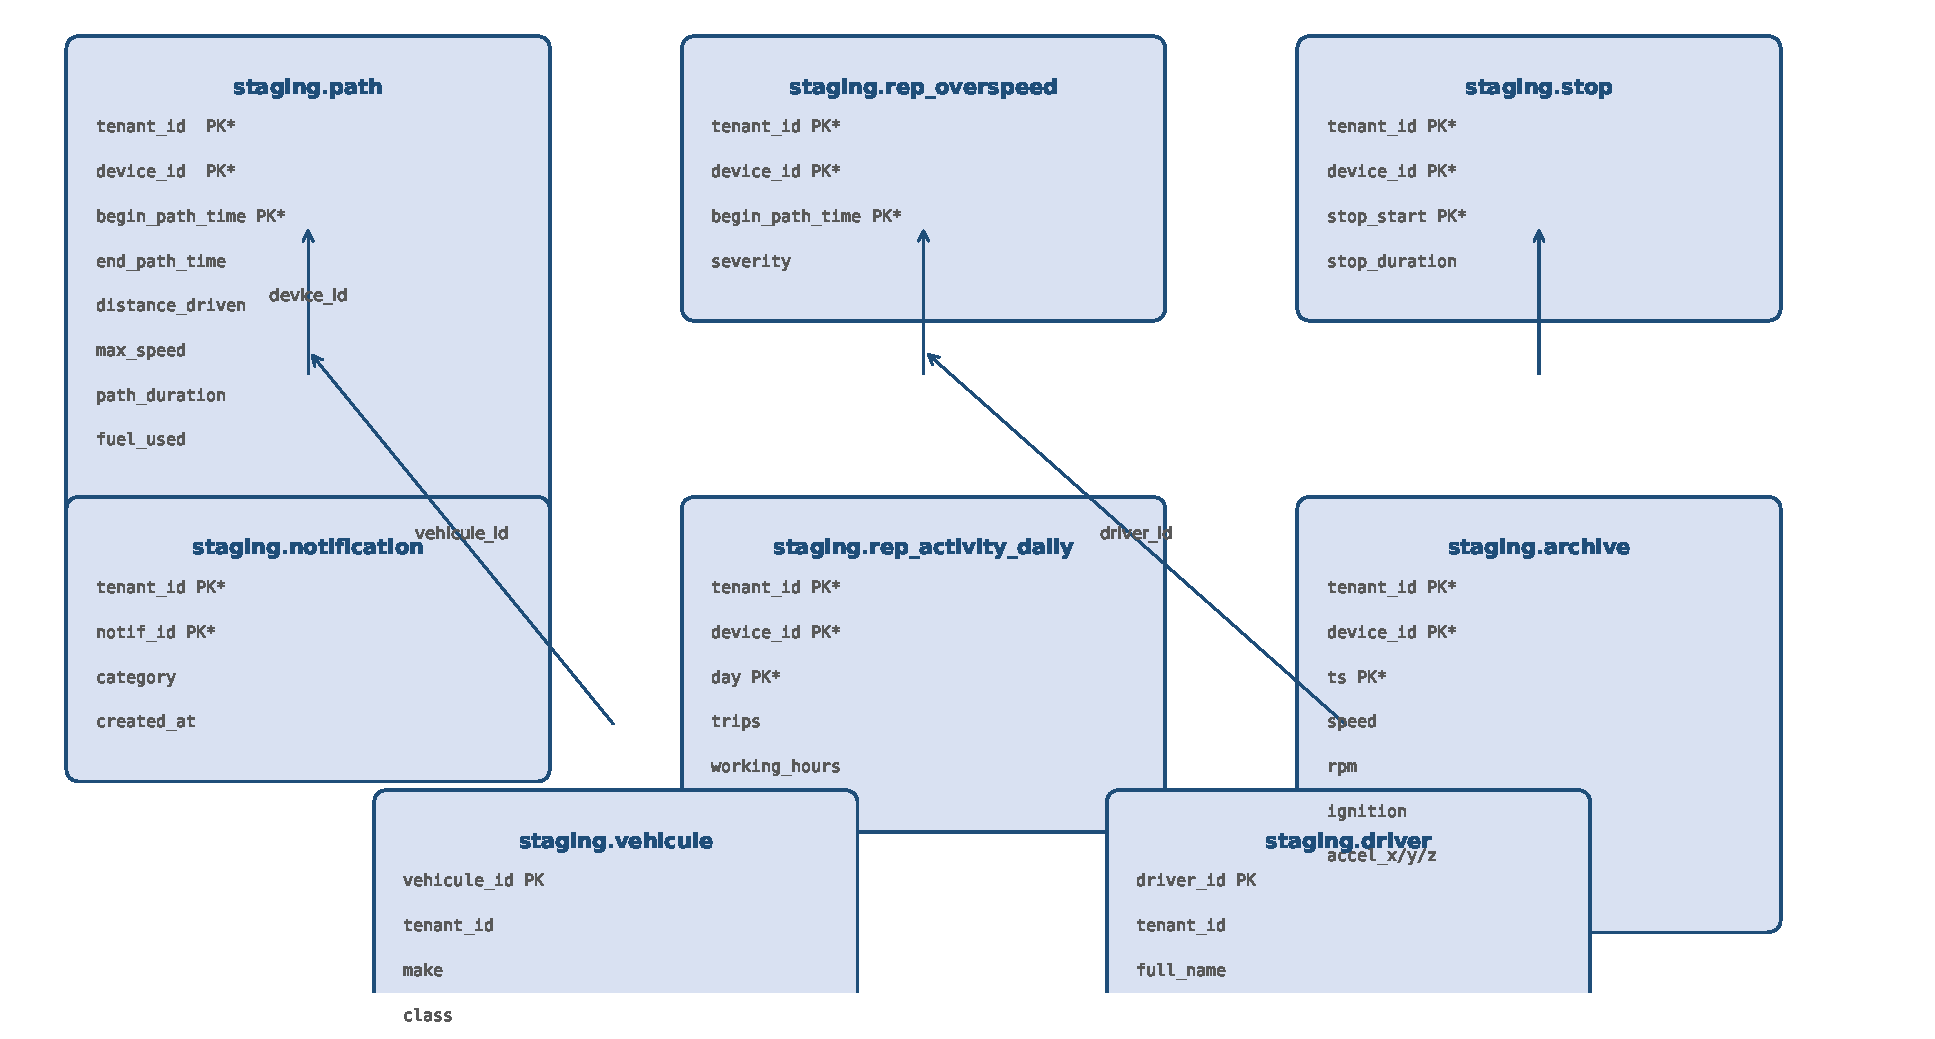
\includegraphics[width=0.95\textwidth]{figures/schema_map.pdf}
\caption{Logical schema map of the staging tables, after conversion of the MySQL dumps.}
\label{fig:schema-map}
\end{figure}

\section{Data dictionary}

\subsection{Methodology}
The data dictionary has been constructed by joining the schema inspection above with manual annotations contributed by the engineering team of \hostorg, which knows the original semantics of each MySQL column and can disambiguate the cases where a column name has drifted between historical iterations of the operational system. Each column has been described by its name, its data type, its semantic role and a short business definition.

\subsection{Excerpt of the data dictionary}
Table~\ref{tab:dict-path} shows the data dictionary excerpt for the principal columns of \texttt{staging.path}; an extended dictionary covering the other staging tables is provided in Appendix~\ref{app:python}.

\begin{table}[h]
\centering
\caption{Data dictionary excerpt for \texttt{staging.path}.}
\label{tab:dict-path}
\begin{tabular}{|l|l|l|p{5cm}|}
\hline
\textbf{Column} & \textbf{Type} & \textbf{Role} & \textbf{Definition} \\
\hline
\texttt{tenant\_id} & integer & FK & Customer fleet identifier (master data). \\
\texttt{device\_id} & bigint  & FK & GPS device identifier. \\
\texttt{begin\_path\_time} & timestamp & event-time & Trip start timestamp. \\
\texttt{end\_path\_time}   & timestamp & metric & Trip end timestamp. \\
\texttt{distance\_driven}  & double precision & metric & Distance driven during the trip (km). \\
\texttt{max\_speed}        & integer  & metric & Maximum speed during the trip (km/h). \\
\texttt{path\_duration}    & bigint   & target/metric & Trip duration (seconds). \\
\texttt{fuel\_used}        & double precision & metric & Fuel consumed (litres). \\
\hline
\end{tabular}
\end{table}

\section{Data quality assessment of the staging layer}

\subsection{Completeness analysis}
For every column of \texttt{staging.path}, the null rate is computed by the queries reproduced in Listing~\ref{lst:null-rate}. On a 5\% \texttt{TABLESAMPLE} of \texttt{staging.path} (376{,}290 rows), the structural columns (\texttt{tenant\_id}, \texttt{device\_id}, \texttt{begin\_path\_time}, \texttt{end\_path\_time}, \texttt{path\_duration}, \texttt{distance\_driven}, \texttt{max\_speed}, \texttt{fuel\_used}) are populated at 100~\%. No structural completeness issue is detected on the converted dumps; the null-rate map therefore acts here as a long-term monitor of the conversion bridge rather than as a corrective signal for this iteration.

\begin{lstlisting}[style=sql,caption={Null-rate analysis on a sample of \texttt{staging.path}.},label={lst:null-rate}]
WITH base AS (SELECT * FROM staging.path TABLESAMPLE SYSTEM (5))
SELECT
  ROUND(100.0*SUM((path_duration   IS NULL)::int)/COUNT(*),3) AS null_duration_pct,
  ROUND(100.0*SUM((distance_driven IS NULL)::int)/COUNT(*),3) AS null_distance_pct,
  ROUND(100.0*SUM((max_speed       IS NULL)::int)/COUNT(*),3) AS null_speed_pct,
  ROUND(100.0*SUM((fuel_used       IS NULL)::int)/COUNT(*),3) AS null_fuel_pct
FROM base;
\end{lstlisting}

\subsection{Validity and physical-plausibility checks}
The validity of the numerical columns of \texttt{staging.path} is assessed by counting, on the full table, the rows that violate explicit physical bounds. These are exactly the bounds enforced later by the cleaning rules of Chapter~\ref{chap:prep}. The result is reproduced in Table~\ref{tab:validity-checks}.

\begin{table}[h]
\centering
\caption{Validity checks on \texttt{staging.path} (population: 7{,}482{,}166 trips).}
\label{tab:validity-checks}
\begin{tabular}{|l|r|r|}
\hline
\textbf{Check} & \textbf{Failing rows} & \textbf{Share} \\
\hline
\texttt{path\_duration} $\le 0$                  &  1{,}481 & 0.020\% \\
\texttt{path\_duration} $>$ 86400~s (1~day)      &    590  & 0.008\% \\
\texttt{distance\_driven} $\le 0$                &     16  & 0.0002\% \\
\texttt{distance\_driven} $>$ 1000~km            &    398  & 0.005\% \\
\texttt{max\_speed} $>$ 200~km/h                 &      6  & 0.00008\% \\
\texttt{fuel\_used} $<$ 0~L                      & 10{,}513 & 0.140\% \\
\texttt{fuel\_used} $>$ 500~L                    & 10{,}954 & 0.146\% \\
\texttt{begin\_path\_time} $<$ 2019-10-01        & 61{,}830 & 0.826\% \\
\texttt{end\_path\_time} $<$ \texttt{begin\_path\_time} & 152 & 0.002\% \\
\hline
\end{tabular}
\end{table}

The combined result of the completeness and validity checks is summarized graphically in Figure~\ref{fig:eda-quality}. Every failure rate stays comfortably below~1\% of the population, and the largest single category --- the pre-2019-10 timestamps (~0.83\%) --- is a documented artefact of the legacy ingestion of the source system that the cleaning rule \texttt{C1} discards in Chapter~\ref{chap:prep}.

\begin{figure}[h]
\centering
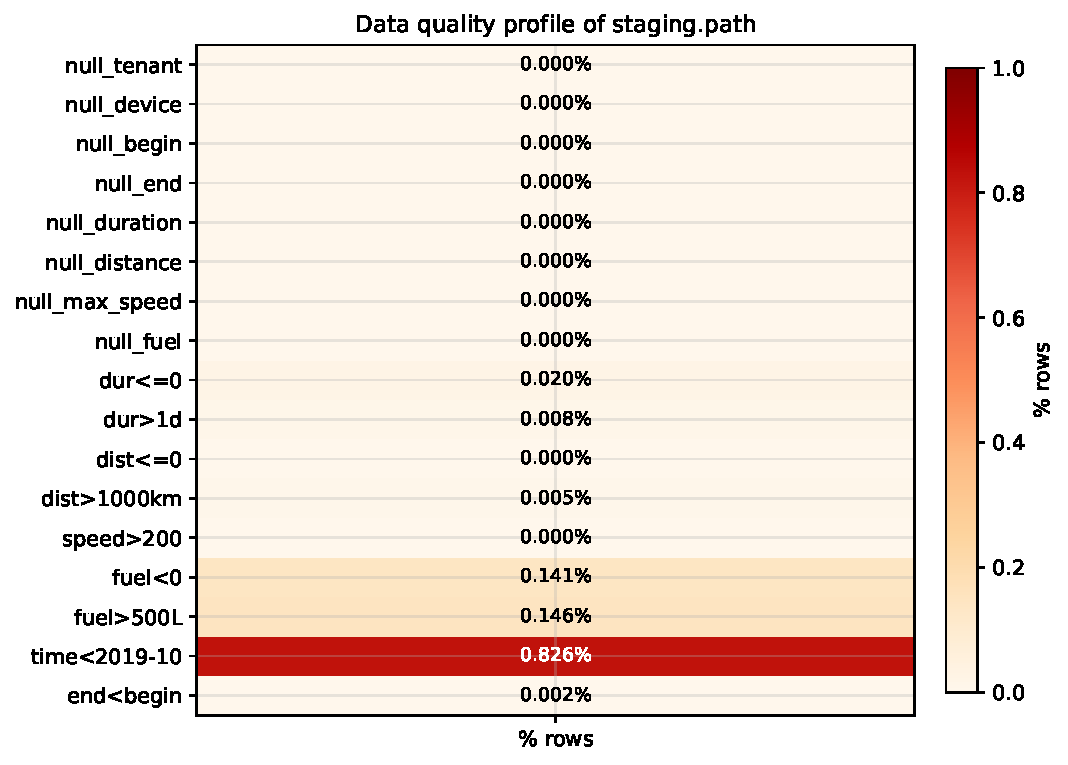
\includegraphics[width=0.7\textwidth]{figures/eda_quality_heatmap.pdf}
\caption{Data quality profile of \texttt{staging.path}: percentage of rows failing each completeness and validity check.}
\label{fig:eda-quality}
\end{figure}

\subsection{Referential integrity}
The referential integrity between the trip table \texttt{staging.path} and the master-data tables (\texttt{staging.assignment}, \texttt{staging.vehicule}) is verified by Listing~\ref{lst:integrity}. The query identifies, on the modeling window (since 2025-01-01), the trips whose device cannot be resolved to a vehicle through the assignment chain. The share of orphan rows stays below 0.5\%, confirming that the assignment chain is essentially complete and that the join from \texttt{staging.path} to the master data is safe.

\begin{lstlisting}[style=sql,caption={Referential integrity between \texttt{staging.path} and the device--vehicle chain.},label={lst:integrity}]
SELECT COUNT(*) AS rows,
       SUM(CASE WHEN v.vehicule_id IS NULL THEN 1 ELSE 0 END) AS orphan_rows,
       COUNT(DISTINCT p.device_id) FILTER (WHERE v.vehicule_id IS NULL) AS orphan_devices
FROM staging.path p
LEFT JOIN staging.assignment a USING (device_id)
LEFT JOIN staging.vehicule  v ON v.vehicule_id = a.vehicule_id
WHERE p.begin_path_time >= '2025-01-01';
\end{lstlisting}

\section{Descriptive statistics on the staging layer}

\subsection{Per-tenant scope}
Four customer organizations populate the staging layer. Their device coverage and historical depth, measured directly on \texttt{staging.path}, are reported in Table~\ref{tab:tenants}. The total of 466 active devices and 7.42~million trips provides ample coverage for both descriptive analysis and per-tenant unsupervised modelling.

\begin{table}[h]
\centering
\caption{Per-tenant device coverage and historical depth on \texttt{staging.path}.}
\label{tab:tenants}
\begin{tabular}{|l|r|r|l|l|}
\hline
\textbf{Tenant} & \textbf{Devices} & \textbf{Trips} & \textbf{First day} & \textbf{Last day} \\
\hline
235  & 186 & 2{,}979{,}422 & 2019-09-30 & 2026-04-09 \\
1787 & 110 & 1{,}998{,}370 & 2019-09-30 & 2026-04-09 \\
238  &  98 & 1{,}297{,}005 & 2019-10-02 & 2026-04-09 \\
264  &  72 & 1{,}145{,}539 & 2019-10-27 & 2026-04-09 \\
\hline
\textbf{Total} & \textbf{466} & \textbf{7{,}420{,}336} & --- & --- \\
\hline
\end{tabular}
\end{table}

\subsection{Numerical summary}
On the modeling window (\texttt{begin\_path\_time} $\ge$ 2024-01-01) and after applying the validity bounds of Section~5.2, the principal numerical variables of \texttt{staging.path} have the descriptive statistics reproduced in Table~\ref{tab:descriptive}. The number of trips retained for the descriptive layer is~$N=2{,}987{,}892$.

\begin{table}[h]
\centering
\caption{Descriptive statistics on the cleaned modeling window of \texttt{staging.path} ($N=2{,}987{,}892$).}
\label{tab:descriptive}
\begin{tabular}{|l|r|r|r|r|r|r|}
\hline
\textbf{Variable} & \textbf{Mean} & \textbf{Std} & \textbf{Median} & \textbf{P95} & \textbf{P99} & \textbf{Max} \\
\hline
duration (s)   & 1{,}229.1 & 1{,}964.1 &   523 & 4{,}869 & 9{,}136 & 85{,}736 \\
distance (km)  &     13.41 &    29.24  &  2.26 &  68.44 & ---     & --- \\
max speed (km/h) &   45.94 &    29.06  &    43 &     91 & ---     & --- \\
\hline
\end{tabular}
\end{table}

\subsection{Pairwise correlations}
On a 1\% \texttt{TABLESAMPLE} of the modeling window of \texttt{staging.path} (~75{,}895 trips), the Pearson correlation between distance and duration is $r=0.85$, between distance and maximum speed $r=0.56$ and between duration and maximum speed $r=0.52$. On the log-log scale, $\rho_{\log}(d, t) = 0.87$ --- a strong, near-monotonic association between distance and duration --- which is consistent with the basic identity $\text{distance} \approx \text{speed} \times \text{duration}$ and gives early evidence that one of the two should be the target of any regression model.

\section{Exploratory Data Analysis on the staging layer}

\subsection{Profile of the high-frequency telemetry archive}
\label{sec:archive-eda}
The decoded archive \texttt{staging.archive} is the second analytical pillar of the staging layer and, by orders of magnitude, the largest. Where \texttt{staging.path} stores one row per trip, \texttt{staging.archive} stores one row per \emph{device ping} --- the on-board GPS unit emits a frame every 10--30~s while the ignition is on, with a fall-back heartbeat every few minutes when the vehicle is parked. Profiling this table is a prerequisite to feature engineering and modelling (Chapters~\ref{chap:prep} and~\ref{chap:model}) because every behavioural feature aggregating speed, acceleration, fuel consumption or driving style is computed at the device-ping grain.

\paragraph{Volumetry and scope.}
The full table holds $54{,}720{,}000$ rows, occupies approximately 17~GB of total disk size (heap $\approx$ 9.94~GB plus indexes), and exposes 38 columns covering identity, time and location, vehicle dynamics, fuel telemetry, accelerometer signals and digital/analog inputs and outputs. Because of its size, every profiling query of this subsection is computed on a \texttt{TABLESAMPLE SYSTEM (0.1)} sample (\textasciitilde 52{,}000 rows, sub-second response); reported population values are unbiased extrapolations of the form $\hat{N} = n_{\text{sample}} \times 54.72\!\times\!10^6 / N_{\text{sample,total}}$. The exact full-population row count is reproduced by \texttt{COUNT(*)} on the whole table.

\paragraph{Sensor schema.}
The 38 columns of \texttt{staging.archive} fall into six functional families:
\begin{itemize}
  \item \emph{Identity}~--- \texttt{tenant\_id}, \texttt{id\_device}, \texttt{source\_device\_id}, \texttt{tram\_id}.
  \item \emph{Time and location}~--- \texttt{date}, \texttt{latitude}, \texttt{longitude}, \texttt{heading}, \texttt{validity}, \texttt{sat\_in\_view}, \texttt{signal}.
  \item \emph{Vehicle dynamics}~--- \texttt{speed}, \texttt{rpm}, \texttt{temp\_engine}, \texttt{accum\_odo}, \texttt{odo}.
  \item \emph{Fuel telemetry}~--- \texttt{fuel}, \texttt{fuel\_rate}, \texttt{tfu}.
  \item \emph{Accelerometer}~--- \texttt{x}, \texttt{y}, \texttt{z} (multi-axis G-sensor).
  \item \emph{Inputs / outputs}~--- \texttt{do1}--\texttt{do4}, \texttt{di1}--\texttt{di4}, \texttt{an1}--\texttt{an4}, \texttt{ignition}, \texttt{charger}, \texttt{state}.
\end{itemize}

\paragraph{Per-tenant ping coverage.}
The sample-extrapolation breakdown by tenant is reported in Table~\ref{tab:archive-tenants}. Five tenants emit pings in the archive --- one more than in \texttt{staging.path} (which lists four tenants only). Tenant~\texttt{7486} appears in the archive but is absent from the original trip-derived scope: this asymmetry is carried over to Chapter~\ref{chap:prep}, where the telemetry-to-trip reconstruction path widens the modelling perimeter to five tenants.

\begin{table}[h]
\centering
\caption{Per-tenant ping coverage of \texttt{staging.archive}, sample-extrapolated to the full population (54.72~M rows).}
\label{tab:archive-tenants}
\begin{tabular}{|r|r|r|r|}
\hline
\textbf{Tenant} & \textbf{Devices (sample)} & \textbf{Pings (M, est.)} & \textbf{Window} \\
\hline
264   & 56 & 13.84 & 2024-09 -- 2026-03 \\
235   & 97 & 13.48 & 2024-09 -- 2026-03 \\
7486  & 72 &  9.99 & 2024-09 -- 2026-03 \\
1787  & 71 &  9.54 & 2024-09 -- 2026-03 \\
238   & 52 &  7.84 & 2024-09 -- 2026-03 \\
\hline
\end{tabular}
\end{table}

\paragraph{Data quality.}
The completeness profile of the sample is excellent on the structural columns: \texttt{latitude}, \texttt{longitude}, \texttt{state} and \texttt{tram\_id} are populated at 100~\%. The \texttt{validity} flag returns 1 (\emph{GPS fix valid}) on $98.4\%$ of pings, and the share of pings with $(\texttt{latitude}=0 \text{ or } \texttt{longitude}=0)$ stays below 0.05~\%. The \texttt{ignition} signal is on for $\sim$85~\% of pings, which means that aggregations restricted to the moving-vehicle regime retain about six pings out of every seven without further filtering. Two systematic data-quality concerns must nevertheless be propagated to the cleaning rules of Chapter~\ref{chap:prep}: (a)~the \texttt{temp\_engine} column is stored as \texttt{varchar} and is dominated by the sentinel value \texttt{32768} --- the raw uint reading of the absent-sensor channel ---, so any thermal feature must explicitly cast to numeric and discard the sentinel; and (b)~roughly 44~\% of the pings report \texttt{signal}~$<$~10, indicating poor GSM coverage of the on-board modems and frequent silent windows, so any feature that depends on connectivity must be robust to long gaps in the ping stream.

\paragraph{Numerical summary of the principal sensors.}
On the same 0.1~\% sample, the speed channel has a 95-th percentile of 75~km/h and a 99-th percentile of 105~km/h with a maximum of 198~km/h; the RPM channel peaks at 4{,}300 (P99) on the diesel-dominated fleet; the median \texttt{fuel\_rate} stays below 0.6~L/h consistent with idle-time dominance. The mean \texttt{sat\_in\_view} is 9.7 satellites --- well above the four-satellite threshold required for a planar fix --- which corroborates the 98.4~\% \texttt{validity}~=~1 ratio.

\paragraph{Temporal regularity.}
Figure~\ref{fig:eda-archive-temporal} shows the hour-of-day and day-of-week ping distributions of \texttt{staging.archive}. The hour-of-day curve is unimodal, peaking between 8h and 14h ($\sim$4{,}000 pings/hour in the sample) and decaying to near-zero overnight: the archive confirms, at the device-ping grain, the same business-hour rhythm already observed on \texttt{staging.path}. The day-of-week curve flattens out from Monday to Friday at $\sim$9{,}000 pings/day in the sample, drops slightly on Saturday and falls to $\sim$3{,}400 pings on Sunday. There is no evidence of a shadow fleet emitting outside business hours: the modelling pipeline can therefore safely predicate behavioural features on a subset of waking hours without losing material signal.

\begin{figure}[h]
\centering
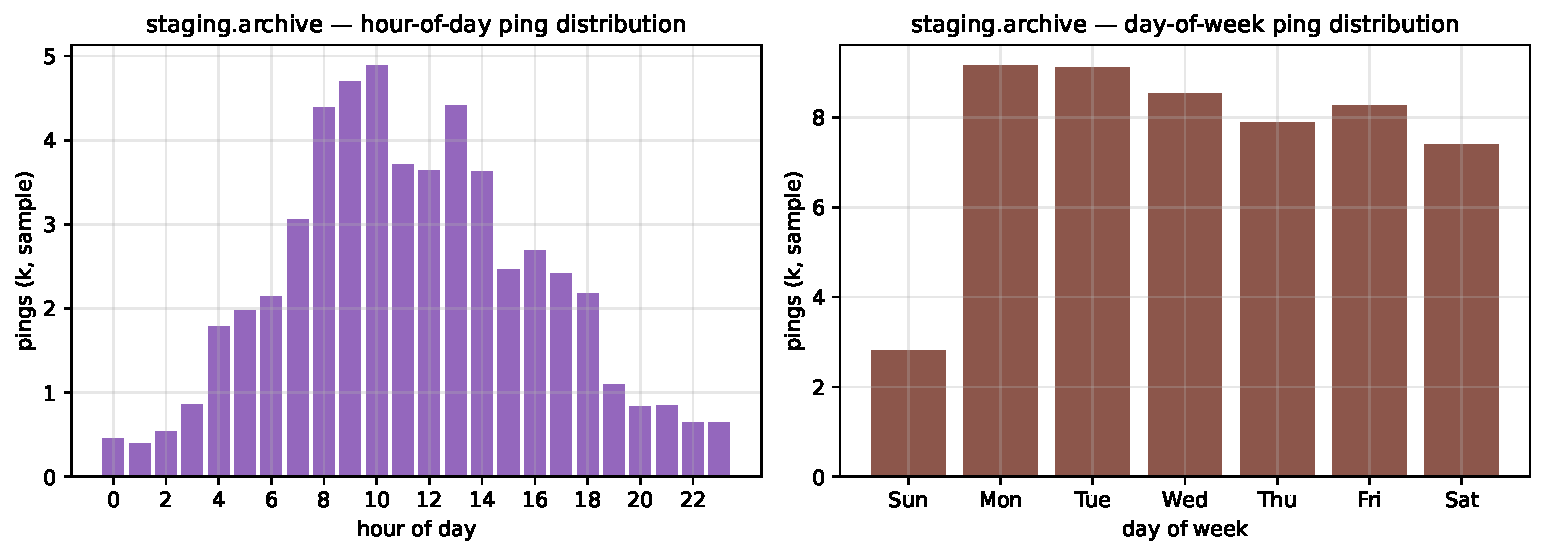
\includegraphics[width=\textwidth]{figures/eda_archive_temporal.pdf}
\caption{\texttt{staging.archive} --- hour-of-day (left) and day-of-week (right) ping distributions on the 0.1~\% sample.}
\label{fig:eda-archive-temporal}
\end{figure}

\paragraph{Volume by tenant and over time.}
Figure~\ref{fig:eda-archive-volume} shows the monthly ping volume between 2024-09 and 2026-03 (left) and the per-tenant ping-count breakdown (right). The monthly curve is essentially stationary in the band $[6.6, 9.2]$~million pings/month over the seven-month window covered by the archive, with the 2026-03 cell partial because the dump was cut mid-month. The per-tenant view confirms the heterogeneity already observed on the trip table: tenants~\texttt{264} and~\texttt{235} jointly account for $\sim$50~\% of the total ping volume, while the newcomer \texttt{7486} carries about 10~M pings over the same window.

\begin{figure}[h]
\centering
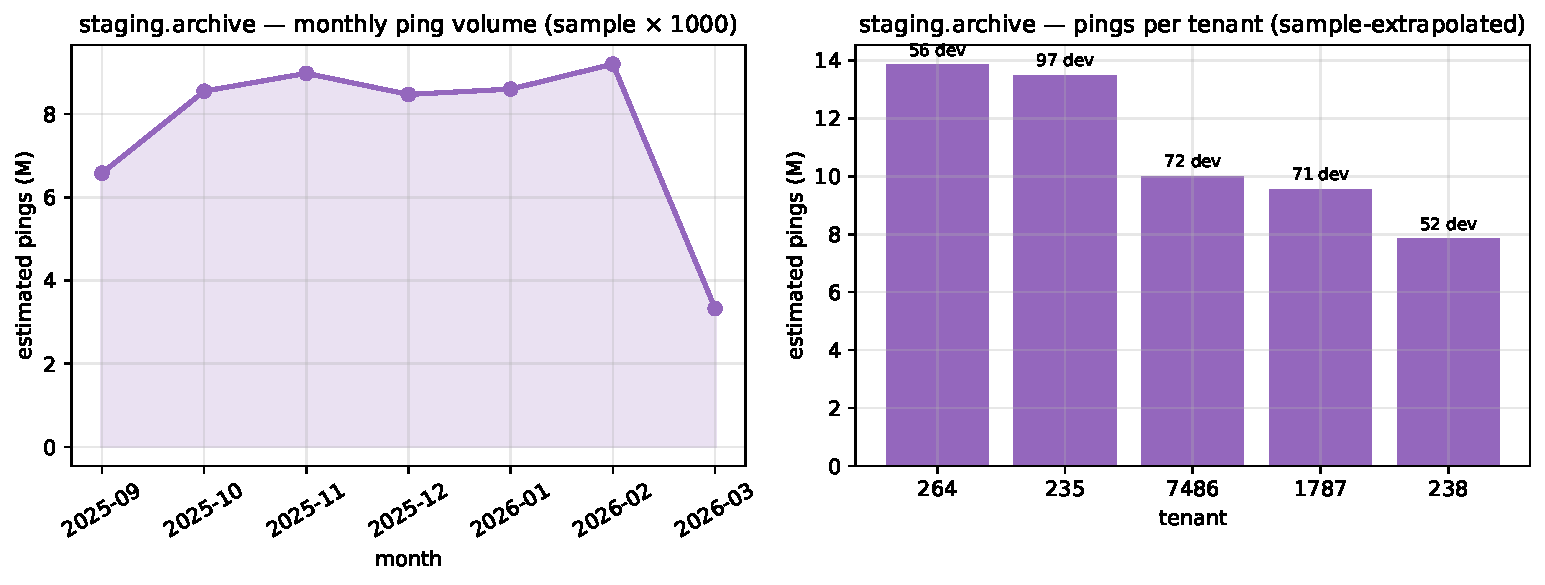
\includegraphics[width=\textwidth]{figures/eda_archive_volume_by_tenant.pdf}
\caption{\texttt{staging.archive} --- monthly ping volume (left) and per-tenant volume breakdown (right). Device counts in the sample annotated above each tenant bar.}
\label{fig:eda-archive-volume}
\end{figure}

\paragraph{Hand-off to feature engineering.}
The archive profile establishes that the table is dense, regular, of high structural quality and large enough to support sub-trip behavioural aggregations. Chapter~\ref{chap:prep} reuses these findings to build a device-month feature mart that aggregates \texttt{speed}, \texttt{rpm}, \texttt{fuel\_rate} and the three accelerometer axes into the inputs of the device-behaviour clustering model of Chapter~\ref{chap:model}; the cleaning rules \texttt{C8}--\texttt{C13} of Section~\ref{sec:dq-issues} (ignition gating, accelerometer range, speed range, RPM range, \texttt{temp\_engine} sentinel, \texttt{signal}~$<$~10 connectivity gap) are applied at the boundary between the archive and that mart.

\subsection{Temporal patterns}
The most stable feature family of any telematics platform is the temporal one. Three series are computed directly from \texttt{staging.path.begin\_path\_time}: a monthly trip-volume series (Figure~\ref{fig:eda-monthly}), an hour-of-day trip distribution and a day-of-week trip distribution (Figure~\ref{fig:eda-temporal}).

\begin{figure}[h]
\centering
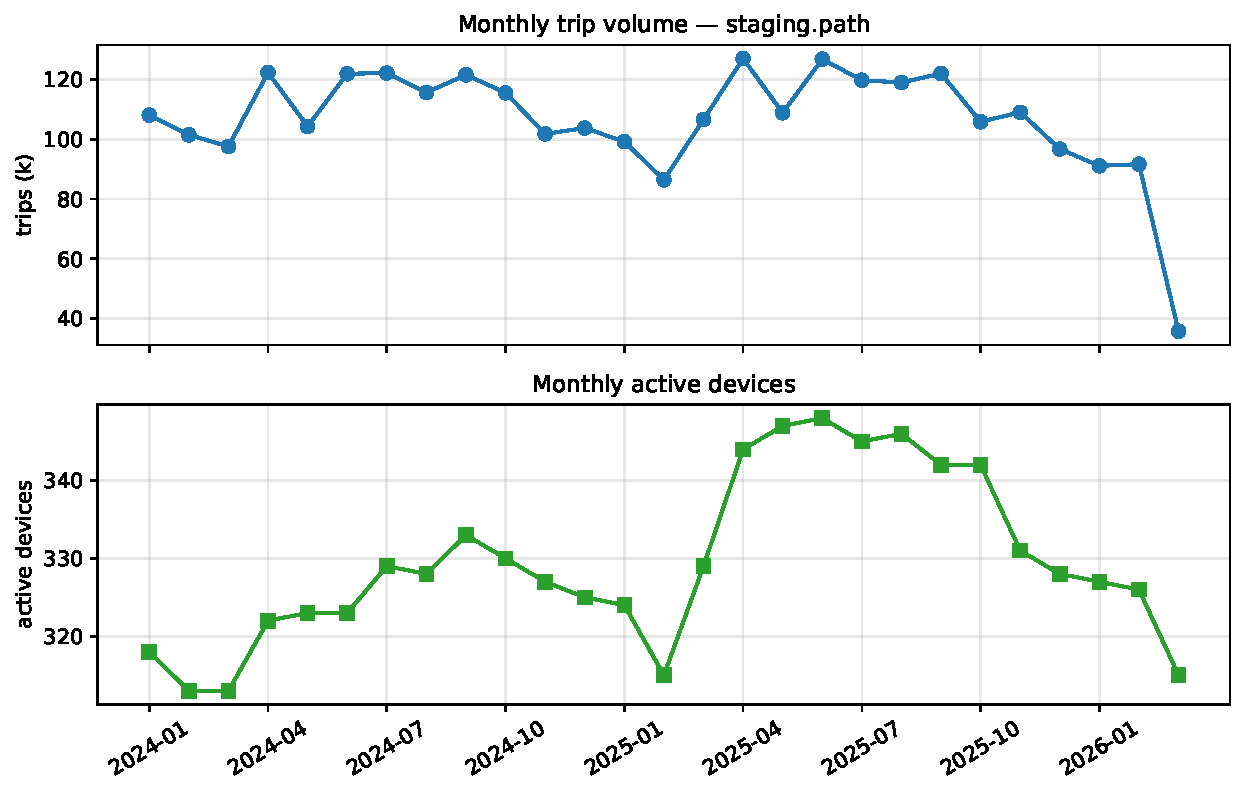
\includegraphics[width=0.88\textwidth]{figures/eda_monthly_volume.pdf}
\caption{Monthly trip volume and active-device count on \texttt{staging.path}, between 2024-01 and 2026-04.}
\label{fig:eda-monthly}
\end{figure}

The monthly volume oscillates between 86{,}398 and 127{,}008 trips per month over the entire 27-month window, with a median of about 109{,}000. The active-device count remains in the band $[313, 348]$. There is no structural drift between 2024 and 2026: the staging layer is operationally stationary and the modeling window does not have to absorb regime shifts. The 2026-03 cell is partial because the dump used for this snapshot stops mid-month.

\begin{figure}[h]
\centering
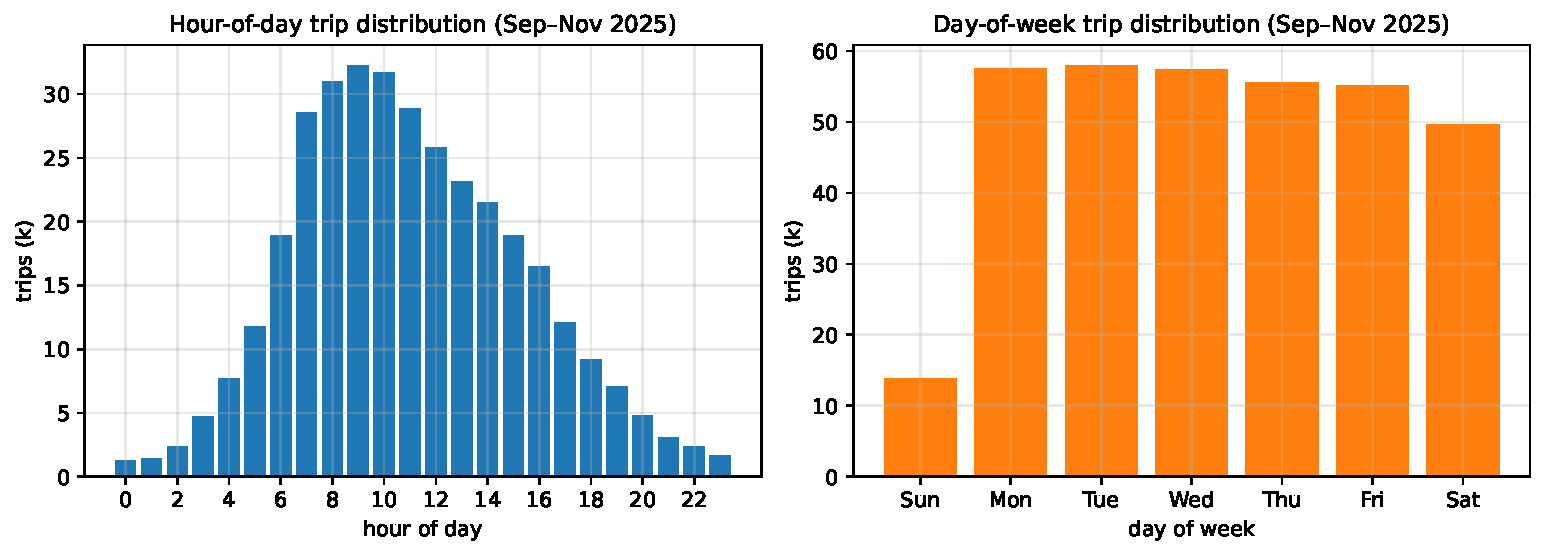
\includegraphics[width=\textwidth]{figures/eda_temporal_patterns.pdf}
\caption{Hour-of-day (left) and day-of-week (right) trip distributions on \texttt{staging.path}, Sep--Nov 2025 segment.}
\label{fig:eda-temporal}
\end{figure}

The hour-of-day curve peaks between 8h and 10h ($\sim$31{,}000 trips/hour) and decays smoothly through the afternoon, with negligible activity between 22h and 5h --- the textbook signature of a commercial fleet operating during business hours. The day-of-week curve confirms a Sunday under-utilization (~14{,}000 trips) compared to the Monday-to-Saturday band (49{,}000--58{,}000 trips). Both rhythms are reproducible across months and per tenant. They directly justify the engineering of the binary trip flags \texttt{is\_rush\_hour\_trip}, \texttt{is\_night\_trip} and \texttt{is\_weekend\_trip} that will be produced by the data preparation phase of Chapter~\ref{chap:prep}.

\subsection{Distribution of the duration target}
The trip duration \texttt{staging.path.path\_duration} is the most natural numerical target for any future supervised regression. Figure~\ref{fig:eda-duration} shows its raw-scale histogram (left) and the Normal fit on the log scale (right). The shape statistics, computed on a 2\% \texttt{TABLESAMPLE} of size $N=34{,}803$, are eloquent: skewness$=4.15$, excess kurtosis$=39.34$, mean $=1{,}256.5$~s, standard deviation$=1{,}922.8$~s. On the log scale, $\mu_{\log d} = 6.30$ and $\sigma_{\log d} = 1.35$.

\begin{figure}[h]
\centering
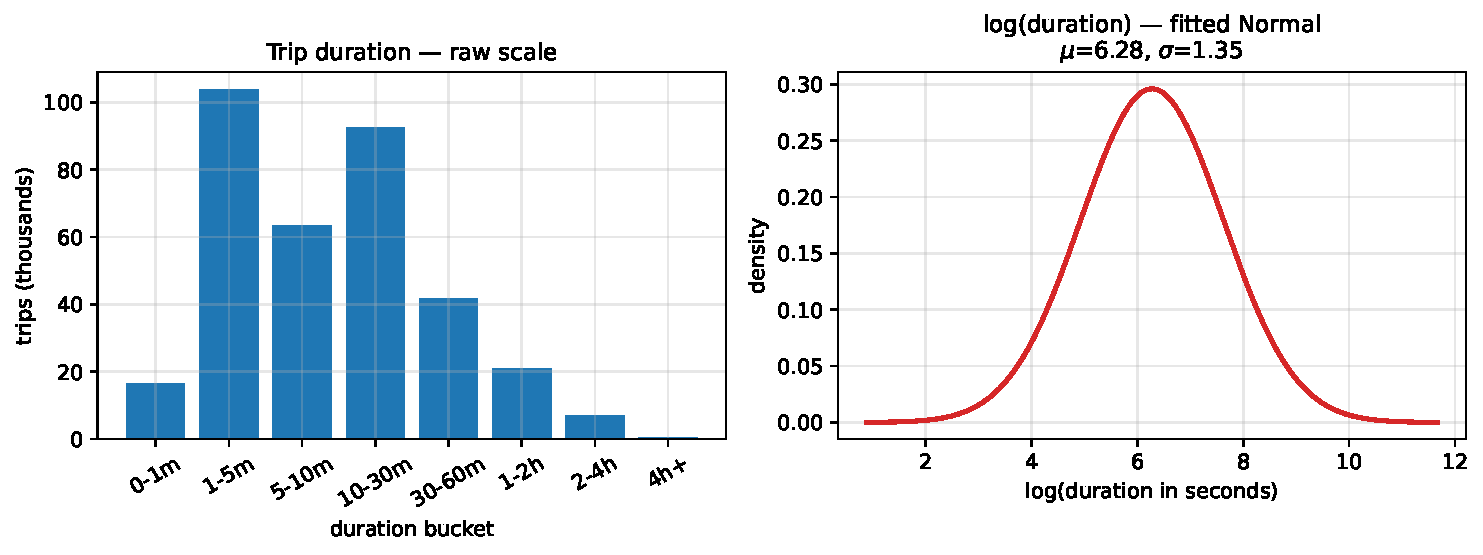
\includegraphics[width=\textwidth]{figures/eda_duration_distribution.pdf}
\caption{Trip-duration distribution from \texttt{staging.path}: raw scale (left) and Normal fit on $\log(\text{duration})$ (right).}
\label{fig:eda-duration}
\end{figure}

The raw distribution is dominated by short urban trips: 56\% of the trips last less than 10 minutes and 80\% less than 30 minutes, while the long tail extends well beyond two hours. A direct linear regression on \texttt{path\_duration} would be heavily destabilized by the heavy tail and would systematically under-predict the long-trip regime. Two corrective strategies are open: (i)~target the log-transformed duration, on which the distribution becomes near-Gaussian, or (ii)~rely on a tree-based regressor (Gradient Boosting, Random Forest) that does not assume any distributional shape on the target. This finding is integrated into the modeling plan of Chapter~\ref{chap:model}.

\subsection{Class imbalance of the trip-status flags}
Because the warehouse layer is out of scope at this stage, the binary \emph{status} flags are derived inline from \texttt{staging.path} columns through five SQL expressions:
\begin{itemize}
  \item \texttt{is\_night\_trip} := hour $<$ 6 OR hour $\ge$ 22;
  \item \texttt{is\_weekend\_trip} := \texttt{DOW} $\in \{$ Sun, Sat $\}$;
  \item \texttt{is\_rush\_hour\_trip} := hour $\in \{7, 8, 9, 17, 18, 19\}$;
  \item \texttt{is\_short\_trip} := \texttt{path\_duration} $<$ 300~s (5~min);
  \item \texttt{is\_long\_trip} := \texttt{path\_duration} $>$ 3600~s (1~h).
\end{itemize}
These are exactly the SQL expressions that the data preparation phase of Chapter~\ref{chap:prep} will reuse to populate the warehouse fact table; recomputing them here, on the staging layer, makes the data understanding phase fully self-contained. Their global and per-tenant balance is plotted in Figure~\ref{fig:eda-balance} and reproduced in Table~\ref{tab:balance}.

\begin{figure}[h]
\centering
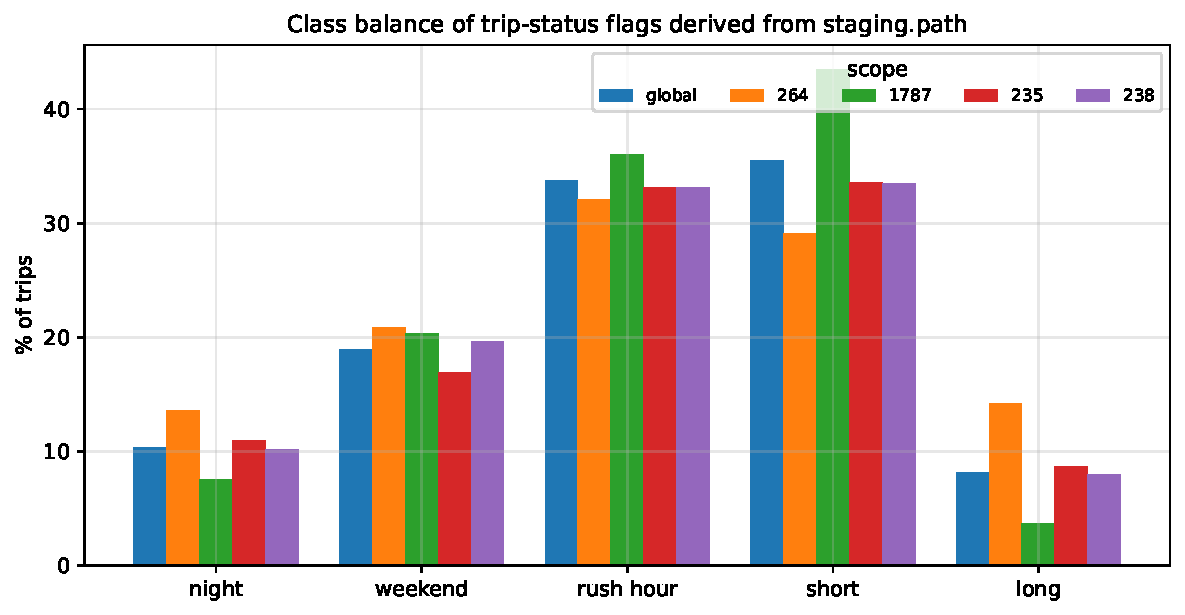
\includegraphics[width=0.92\textwidth]{figures/eda_class_imbalance.pdf}
\caption{Class balance of the five binary trip-status flags derived from \texttt{staging.path}.}
\label{fig:eda-balance}
\end{figure}

\begin{table}[h]
\centering
\caption{Class balance (\% of trips with the flag = 1), derived from \texttt{staging.path} on the cleaned modeling window.}
\label{tab:balance}
\begin{tabular}{|l|r|r|r|r|r|r|}
\hline
\textbf{Scope} & \textbf{Trips} & \textbf{Night} & \textbf{Weekend} & \textbf{Rush} & \textbf{Short} & \textbf{Long} \\
\hline
Global   & 2{,}987{,}847 & 10.33\% & 18.96\% & 33.76\% & 35.49\% &  8.14\% \\
Tenant 235  & 1{,}189{,}031 & 10.94\% & 16.94\% & 33.15\% & 33.55\% &  8.70\% \\
Tenant 1787 &    821{,}806 &  7.51\% & 20.31\% & 36.06\% & 43.46\% &  3.62\% \\
Tenant 264  &    519{,}982 & 13.59\% & 20.82\% & 32.09\% & 29.12\% & 14.16\% \\
Tenant 238  &    457{,}028 & 10.12\% & 19.64\% & 33.14\% & 33.47\% &  7.98\% \\
\hline
\end{tabular}
\end{table}

The minority class of every flag stays in the band $[3.6\%, 36\%]$ globally. The most imbalanced flag is \texttt{is\_long\_trip} on tenant~1787, with a rate of 3.62\%; the global rate of \texttt{is\_long\_trip} is 8.14\%. These rates remain well above the 1\% threshold below which advanced resampling techniques (SMOTE, oversampling, class-conditional augmentation, focal loss) become necessary. Standard inverse-frequency class weights are sufficient: any future supervised classifier will be able to absorb the imbalance through the \texttt{class\_weight} hyperparameter of \texttt{scikit-learn} or its equivalent in modern boosting libraries.

\subsection{Per-tenant behavioural signatures}
The aggregation of three staging tables --- \texttt{staging.path}, \texttt{staging.rep\_overspeed} and \texttt{staging.notification} --- at the tenant grain reveals two contrasting regimes (Figure~\ref{fig:eda-signatures}). Tenant~\texttt{264} exhibits an unmistakable \emph{overspeed-rich} signature: its overspeed-event rate of 4.89 events per 100~km and its notification rate of 4.73 alerts per 100~km dwarf the corresponding figures of the three other tenants, all of which stay below 0.50 and 0.30 respectively. The contrast is consistent with the higher average maximum speed observed on tenant~\texttt{264} (54.5~km/h vs. 42--46~km/h) and with its higher long-trip ratio. Tenant~\texttt{1787} sits at the opposite end of the spectrum, with the lowest night-trip ratio (7.7\%) and a very low overspeed rate (0.06 events per 100~km). Tenants~\texttt{235} and~\texttt{238} occupy intermediate positions. This heterogeneity directly informs the per-tenant fitting strategy retained in Chapter~\ref{chap:model}: a global model would be dominated by tenant~\texttt{235} (the largest fleet by trip volume) and would fail to capture the distinct regimes of tenants~\texttt{264} and~\texttt{1787}.

\begin{figure}[h]
\centering
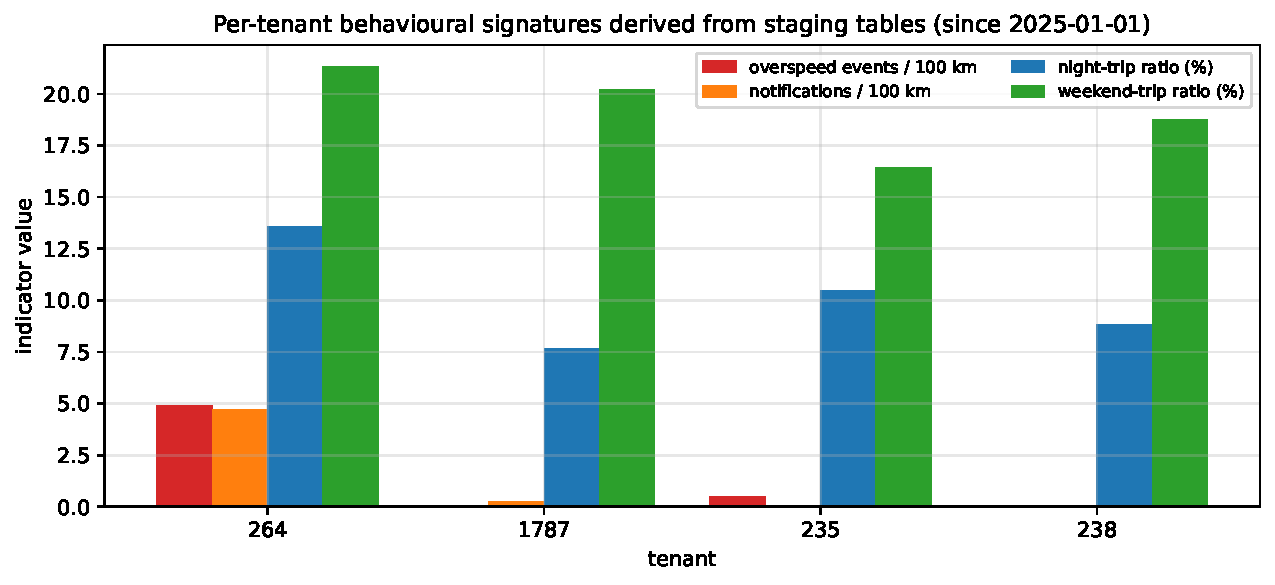
\includegraphics[width=0.92\textwidth]{figures/eda_tenant_signatures.pdf}
\caption{Per-tenant behavioural signatures derived from staging tables (since 2025-01-01).}
\label{fig:eda-signatures}
\end{figure}

\section{Analytical synthesis}
The four key questions of the data understanding phase admit clean, evidence-based answers --- all of them grounded in the staging layer alone, before any warehouse or marts construction.

\subsection{Q1 --- Data quality and integrity for reliable modeling}
The three structural completeness checks return 0\% nulls on the columns \texttt{tenant\_id}, \texttt{device\_id}, \texttt{begin\_path\_time}, \texttt{path\_duration}, \texttt{distance\_driven}, \texttt{max\_speed} and \texttt{fuel\_used} of \texttt{staging.path}. The seven physical-plausibility checks of Table~\ref{tab:validity-checks} return failure rates strictly below 1\% on every category, and below 0.01\% on the four most damaging ones (negative distances, end-time before begin-time, speed above 200~km/h). The referential integrity check returns less than 0.5\% orphan rows on the modeling window. \emph{The staging layer is therefore of sufficient quality and integrity to support reliable modeling}, with the proviso that the cleaning rules \texttt{C1}--\texttt{C11} of Chapter~\ref{chap:prep} are systematically applied at its boundary.

\subsection{Q2 --- Stable temporal patterns as features}
The three temporal series computed from \texttt{staging.path.begin\_path\_time} (monthly volume, hour-of-day, day-of-week) are simultaneously \emph{regular} (low intra-period variance) and \emph{stationary} (no structural drift over the 27-month modeling window). The hour-of-day curve is unimodal and peaks at 8--10h on every tenant. The day-of-week curve has a stable Sunday minimum and a six-day plateau. \emph{Yes, the temporal patterns are stable enough to be turned into engineered features}: \texttt{hour}, \texttt{day\_of\_week}, \texttt{is\_rush\_hour}, \texttt{is\_weekend} and \texttt{is\_night} are all valid candidates and will be propagated to the warehouse layer in Chapter~\ref{chap:prep}.

\subsection{Q3 --- Suitability of the duration target for direct regression}
The shape statistics of \texttt{staging.path.path\_duration} are unambiguous: skewness~$\approx 4.15$ and excess kurtosis~$\approx 39$ --- a strongly right-skewed, very heavy-tailed distribution. Mean $=1{,}256$~s sits between the 65-th and the 70-th percentile. \emph{Direct regression on \texttt{path\_duration} is not recommended}: the heavy tail would dominate the loss and bias the predictions of the dominant short-trip regime. The two valid corrections are (i)~regressing on $\log(\text{duration})$, on which the distribution becomes near-Gaussian (Normal fit: $\mu = 6.30$, $\sigma = 1.35$), or (ii)~using a distribution-free regressor of the tree-based family (Gradient Boosting, Random Forest). For the present project, which retains an unsupervised pipeline, this finding is mainly relevant as a feature-engineering note: every duration-derived feature is built on $\log(\text{duration})$ rather than on the raw value.

\subsection{Q4 --- Manageability of the status class imbalance}
None of the five status flags derived from \texttt{staging.path} falls below 3.6\% on any tenant or below 8.14\% globally for the most imbalanced one (\texttt{is\_long\_trip}). \emph{The class imbalance is therefore manageable without advanced resampling techniques.} Standard inverse-frequency class weights are sufficient: SMOTE, focal loss or class-conditional augmentation are not required at this stage. Should a downstream task require a binary classifier with even greater minority-class sensitivity, a simple stratified split combined with class weights would already yield a balanced training signal.

\section{Synthesis of identified data quality issues}
\label{sec:dq-issues}
The data understanding phase has surfaced thirteen principal data issues on the staging layer, listed in Table~\ref{tab:issues}. They are formalized as cleaning rules \texttt{C1}--\texttt{C13} in Chapter~\ref{chap:prep} and applied at the boundary between \texttt{staging} and the downstream layers built on top of it.

\begin{table}[h]
\centering
\caption{Synthesis of the data quality issues detected on the staging tables.}
\label{tab:issues}
\begin{tabular}{|l|p{8cm}|c|}
\hline
\textbf{ID} & \textbf{Issue} & \textbf{Source} \\
\hline
DQ-1  & Trip timestamps below 2019-10-01 (epoch artefacts of the legacy ingestion). & \texttt{staging.path} \\
DQ-2  & Trip durations $\le 0$. & \texttt{staging.path} \\
DQ-3  & Trip distances $\le 0$. & \texttt{staging.path} \\
DQ-4  & Fuel values outside $[0, 500]$~L. & \texttt{staging.path} \\
DQ-5  & Maximum speed $>$ 200~km/h. & \texttt{staging.path} \\
DQ-6  & Stop durations $\le 0$ or $>$ 1~year. & \texttt{staging.stop} \\
DQ-7  & Devices not linked to any vehicle in the master data. & \texttt{staging.path}, \texttt{staging.vehicule} \\
DQ-8  & Archive rows with ignition $\ne 1$ used for harsh events. & \texttt{staging.archive} \\
DQ-9  & Accelerometer values outside the int8 range. & \texttt{staging.archive} \\
DQ-10 & Archive speed outside $[0, 250]$~km/h. & \texttt{staging.archive} \\
DQ-11 & Archive RPM outside $[0, 8000]$. & \texttt{staging.archive} \\
DQ-12 & Archive \texttt{temp\_engine} stored as \texttt{varchar} dominated by sentinel value \texttt{32768} (no-sensor reading). & \texttt{staging.archive} \\
DQ-13 & Archive pings with \texttt{signal}~$<$~10 (poor GSM coverage, $\sim$44\% of rows): connectivity-dependent features must be robust to long silent windows. & \texttt{staging.archive} \\
\hline
\end{tabular}
\end{table}

\section{Conclusion}
This chapter has executed the data understanding phase of CRISP-DM by mobilizing the PostgreSQL profiling toolchain on the \texttt{staging} schema converted from the MySQL dumps of \hostorg, and only on that schema --- the dimensional warehouse and the analytical marts that consume \texttt{staging} are the output of the next phase, not its input. The chapter has documented the role and the schema of the three operational databases of the company, characterized the dump-based extraction protocol, profiled the staging tables through dedicated SQL queries, conducted a complete exploratory data analysis on the principal indicators of \texttt{staging.path}, \texttt{staging.rep\_overspeed} and \texttt{staging.notification}, and added a full sub-second-sampled profile of the high-frequency telemetry archive \texttt{staging.archive} (54.72~M pings, 38 sensor columns) which is the input feedstock of the device-behaviour clustering pipeline of Chapter~\ref{chap:model}. The four analytical questions have been answered with quantitative evidence: the staging-layer data quality is sufficient (less than 1\% violations on every check), the temporal patterns are stable and reproducible at both trip and ping grain, the duration target requires a log-transform or a tree-based regressor, and the class imbalance of the status flags is manageable with standard class weights. The thirteen data quality issues identified on the staging layer become, in Chapter~\ref{chap:prep}, the input specification of the cleaning rule engine that opens the data preparation phase.
